\documentclass[11pt]{article}
\usepackage[utf8]{inputenc}
\usepackage{amsmath,amsthm,amsfonts,amssymb,amscd}
\usepackage{multirow,booktabs}
\usepackage{enumitem}
\usepackage{fancyhdr}
\usepackage{mathrsfs}
\usepackage{wrapfig}
\usepackage{setspace}
\usepackage{calc}
\usepackage{multicol}
\usepackage{cancel}
\usepackage[retainorgcmds]{IEEEtrantools}
\usepackage{framed}
\usepackage[most]{tcolorbox}
\usepackage{tikz}
\usepackage{geometry}
\geometry{
	a4paper,
	total={170mm,257mm},
	left=20mm,
	top=20mm,
}
\title{Electromagnetic Waves}
\author{Aaron G.K.}
\begin{document}
\maketitle
\section*{Maxwell's Laws and Theory of Electromagnetism}
All light - we humans are able to observe and not able to are made of electromagnetic waves. These electromagnetic waves were first theorized by the brilliant 19th Century scientist James Clerk Maxwell. Maxwell brought together all the work that had been done by brilliant physicists such as Oersted, Coulomb, Gauss, and Faraday, and added his own insights to develop the overarching theory of electromagnetism. Maxwell’s equations require some vector calculus to understand, so we will discuss each law by explaining the physical phenomena they are associated with. Maxwell's equations are good not only because they were elegantly simple, but also because they showed symmetry in nature and math.
\begin{enumerate}
	\item Electric field lines originate on positive charges and terminate on negative charges. The electric field is defined as the force per unit charge on a test charge, and the strength of the force is related to the electric constant. This is also known as Gauss’s law for electricity.
	\item Magnetic field lines are continuous, having no beginning or end. No magnetic monopoles are known to exist. The strength of the magnetic force is related to the magnetic constant. This law is known as Gauss’s law for magnetism.
	\item Magnetic fields are generated by moving charges or by changing electric fields. This law encompasses Ampere’s law.
	\item A changing magnetic field induces an electromotive force (emf) and, hence, an electric field. The direction of the emf opposes the change. This is Faraday’s law of induction, and includes Lenz’s law.
\end{enumerate}
Maxwell’s theory, being symmetric, showed that electric and magnetic forces are not different, but different manifestations of the same thing—the electromagnetic force.\\ \\
Since changing electric fields create relatively weak magnetic fields(that was one of Maxwell's propositions), they could not be easily detected at the time of Maxwell’s hypothesis. Maxwell realized, however, that oscillating charges, like those in AC circuits, produce changing electric fields. He predicted that these changing fields would propagate from the source like waves generated on swimming pool from a diver jumping into the pool. The waves predicted by Maxwell would consist of oscillating electric and magnetic fields — defined to be an electromagnetic wave. Maxwell calculated that electromagnetic waves would propagate at a speed given by the equation $c = \dfrac{1}{\sqrt{\mu_{0}\epsilon_{0}}}$. We can plug in the values for electric and magnetic constants and we would approximately get the value of $c=3.00\times10^8m/s$ which is the speed of light in vacuum. Maxwell proposed that light was an electromagnetic wave and there were other waves that were not visible to the human eye. Sadly, the experimental proof came after Maxwell had passed away.
\subsection*{Experimental Proof for Existence of EM Waves}
Heinrich Hertz was the first to generate and detect certain types of electromagnetic waves in the laboratory. He performed a series of experiments that not only confirmed the existence of electromagnetic waves, but also verified that they travel at the speed of light. He had a simple setup of an RLC circuit and a tuner as shown in the figure below.
\begin{center}
	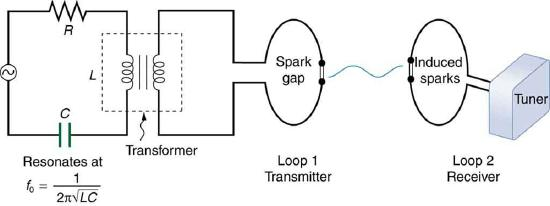
\includegraphics[scale=0.6]{rlc}
\end{center}
An RLC circuit connected to the first loop caused sparks across a gap in the wire loop and generated electromagnetic waves. Sparks across a gap in the second loop located across the laboratory gave evidence that the waves had been received. Hertz also studied the reflection, refraction, and interference patterns of the electromagnetic waves he generated, verifying that they are indeed waves. He was able to determine wavelength from the interference patterns, and knowing their frequency, he could calculate the propagation speed using the equation $v=f\lambda$. Hertz was thus able to prove that electromagnetic waves travel at the speed of light. The SI unit for frequency, the hertz ( 1Hz=1cycle/sec), is named is his honor.
\subsection*{Producing and Propagating EM Waves}
For simplicity, let's assume there is a straight current carrying wire with an AC current through it. A changing current produces both an Electric Field and a Magnetic Field. Since the current is changing, the accompanying electric and magnetic fields are changing which propagate away from the source at the speed of light in vacuum.
\begin{center}
	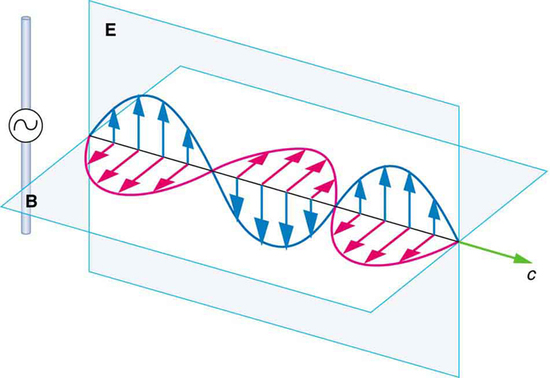
\includegraphics[scale=0.8]{em_wave}
\end{center}
The basic working principle behind antennas is the concept we just saw above. A charge accelerates and it radiates electric and magnetic fields that are in sync (and perpendicular). In radio and TV antennas for instance, the signal is created at the station and transmitted through a large antenna while we have smaller antennas in the house to receive the signal; these receiver antennas are specially designed to resonate at particular frequencies. An incoming electromagnetic wave accelerates electrons in the antenna, setting up a standing wave. If the radio or TV is switched on, electrical components pick up and amplify the signal formed by the accelerating electrons. The signal is then converted to audio and/or video format. Sometimes big receiver dishes are used to focus the signal onto an antenna. \\ \\
For the same source, the magnetic field and electric field are directly proportional. As the current increases the magnetic field increases and so does the electric field. And when the current decreases, both the electric and magnetic fields decrease. However, we can relate the electric and magnetic field strengths of an electromagnetic wave and it is as follows;
$$\vec{E}=c\vec{B}\text{ such that }c=3.00\times10^8m/s$$  
\section*{The Electromagnetic Spectrum}
We mainly classify the electromagnetic waves based on the range of frequencies/wavelengths they occur in but since some might overlap in their ranges, we use the sources of the waves to identify which kinds they are. Something very unique or counterintuitive about EM waves is that when the waves encounter an object in their path, it is possible to have partial transmission, reflection, and absorption. We normally associate these properties with visible light, but they do apply to all electromagnetic waves. What is not obvious is that something that is transparent to light may be opaque at other frequencies. For example, ordinary glass is transparent to visible light but largely opaque to ultraviolet radiation. Human skin is opaque to visible light -- we cannot see through people -- but transparent to X-rays. \\ \\
Since all electromagnetic waves travel at the speed of light in vacuum, their frequencies and wavelengths are inversely proportional.
$$c=\lambda f\implies f=\dfrac{c}{\lambda}\implies \lambda=\dfrac{c}{f}$$
Thus, the higher the frequency of an EM wave, the lower its wavelength and the higher its wavelength, the lower frequency it has.
\begin{center}
	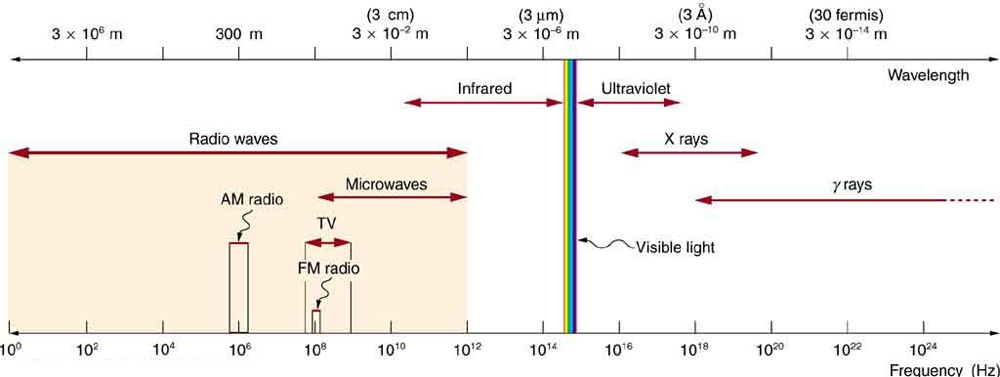
\includegraphics[scale=0.8]{em_spectrum}
\end{center}
\subsubsection*{Radio Waves}
\begin{center}
	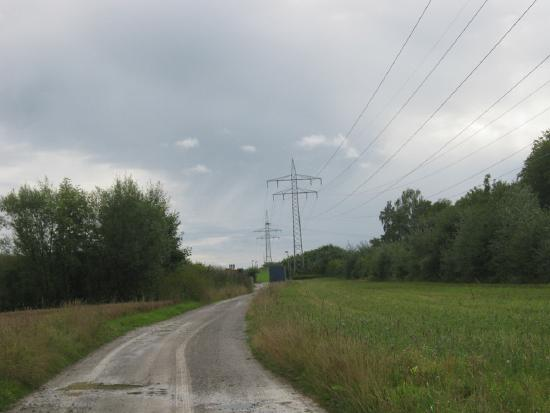
\includegraphics[scale=0.3]{radio}
\end{center}
These waves are the waves that are bottom frequency end of the spectrum. They have less frequency \& energy than the other EM waves, however, they have much larger wavelengths which makes them ideal in communications. Radio waves are produced by accelerating charges. Radio waves have a range of applications including communications between people on land and submarines by making use of Extremely Low Frequency(ELF) waves that have very large wavelengths and are able to travel larger distances more. We can use radio waves by varying the amplitude(AM) and/or frequency(FM) on our receiver antenna. \\ \\
Astronomers collect signals from outer space mostly using electromagnetic waves. A common problem for astrophysicists is the “dust” from electromagnetic radiation pervading our surroundings from communication systems in general. In order to prevent interference between all these electromagnetic signals, strict regulations are drawn up for different organizations to utilize different radio frequency bands.
\subsubsection*{Microwaves}
\begin{center}
	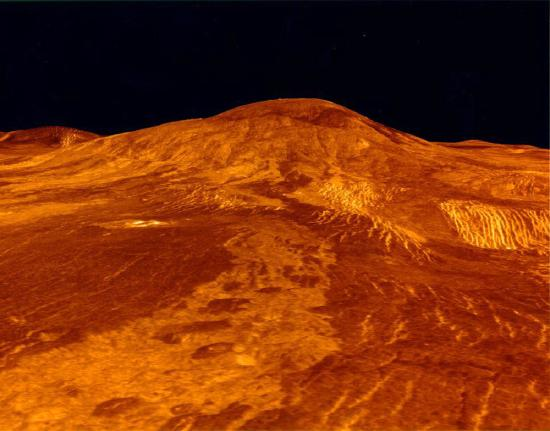
\includegraphics[scale=0.3]{microwave}
\end{center}
Microwaves are waves that have frequencies larger than radio waves and are made by accelerating charges and thermal agitation of matter - in fact, they are waves that have the highest frequency to be made using macroscopic circuits \& devices. Since it is possible to carry more information per unit time on high frequencies, microwaves are more suitable for communications than radio waves. Most satellite-transmitted information is carried on microwaves, as are land-based long-distance transmissions. \\ \\
Another important use of microwaves is in microwave ovens. Water and some other constituents of food have a slightly negative charge at one end and a slightly positive charge at the other end. The range of microwave frequencies is specially selected so that the polar molecules, in trying to keep orienting themselves with the electric field, absorb these energies and increase their temperatures. The energy thereby absorbed results in thermal agitation heating food and not the plate, which does not contain water. Hot spots in the food are related to constructive and destructive interference patterns. Rotating antennas and food turntables help spread out the hot spots. \\ \\
Deep space also acts like a blackbody with a 2.7 K temperature, radiating most of its energy in the microwave frequency range. In the mid 20th Century, Penzias and Wilson detected this radiation and eventually recognized that it was the radiation of the Big Bang’s cooled remnants.
\subsubsection*{Infrared Radiation}
\begin{center}
	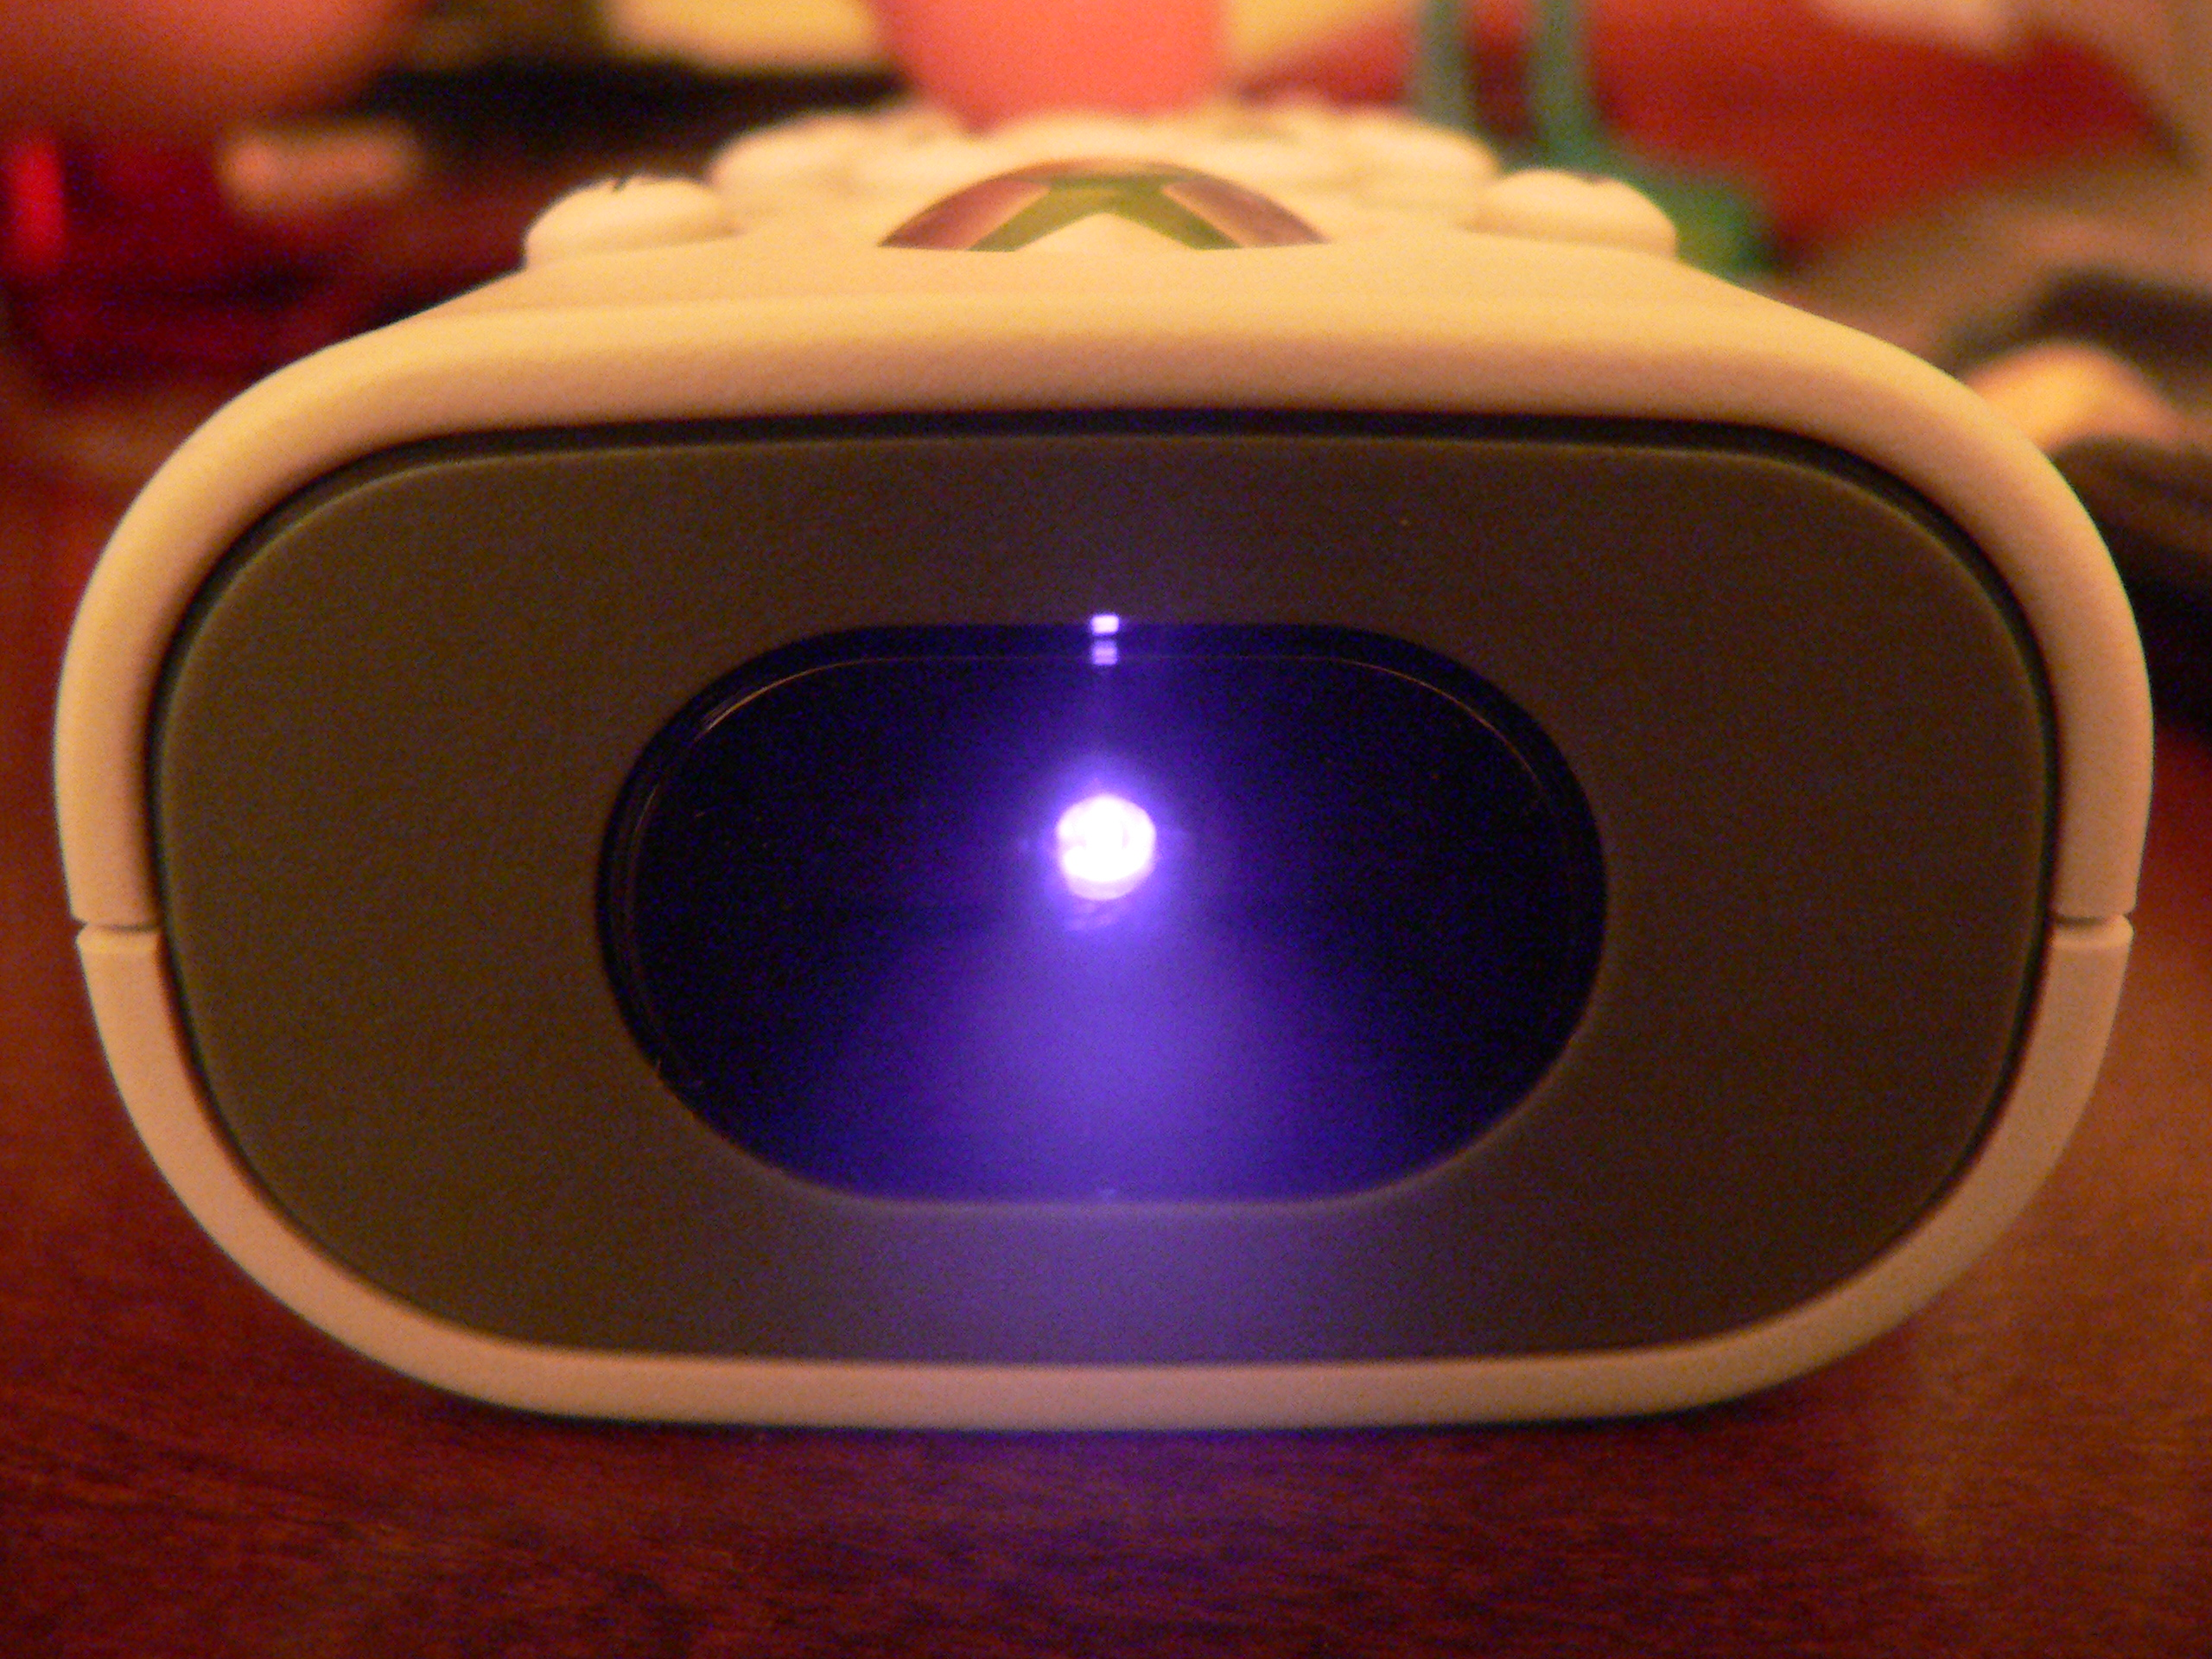
\includegraphics[scale=0.05]{infrared}
\end{center}
Infrared radiation is generally produced by thermal motion and the vibration and rotation of atoms and molecules. Electronic transitions in atoms and molecules can also produce infrared radiation. \\ \\
The range of infrared frequencies extends up to the lower limit of visible light, just below red. In fact, infrared means “below red.” Frequencies at its upper limit are too high to be produced by accelerating electrons in circuits, but small systems, such as atoms and molecules, can vibrate fast enough to produce these waves. We can study radiant heat transfer from a house by using a camera capable of detecting infrared radiation. Some satellites can detect buildings, vehicles, and even individual humans by their infrared emissions, whose power radiation is proportional to the fourth power of the absolute temperature. More mundanely, we use infrared lamps, some of which are called quartz heaters, to preferentially warm us because we absorb infrared better than our surroundings.
\subsubsection*{Visible Light}
\begin{center}
	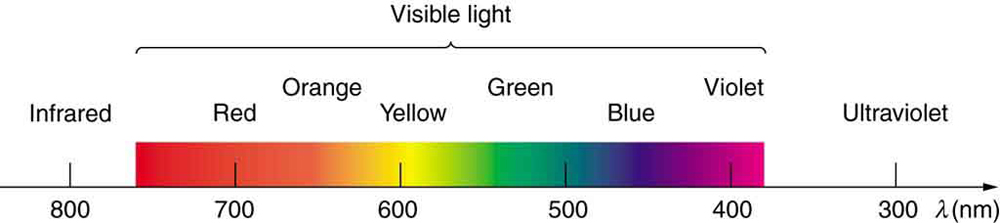
\includegraphics[scale=0.5]{vl}
\end{center}
Visible light is the segment of the electromagnetic spectrum to which the human eye responds. Visible light is produced by vibrations and rotations of atoms and molecules, as well as by electronic transitions within atoms and molecules. The receivers or detectors of light largely utilize electronic transitions. We say the atoms and molecules are excited when they absorb and relax when they emit through electronic transitions. \\ \\
The picture at the top shows this part of the spectrum, together with the colors associated with particular pure wavelengths. We usually refer to visible light as having wavelengths of between 400 nm and 750 nm. (The retina of our eye actually responds to the lowest ultraviolet frequencies, but these do not normally reach the retina because they are absorbed by the cornea and lens of the eye.) Red light has the lowest frequencies and longest wavelengths, while violet has the highest frequencies and shortest wavelengths. 
Living things have evolved to utilize and respond to parts of the electromagnetic spectrum they are embedded in. Visible light is the most predominant and we enjoy the beauty of nature through visible light. Plants and other photosynthetic organisms are more selective. Photosynthesis makes use of parts of the visible spectrum to make sugars.
\subsubsection*{Ultraviolet Radiation}
\begin{center}
	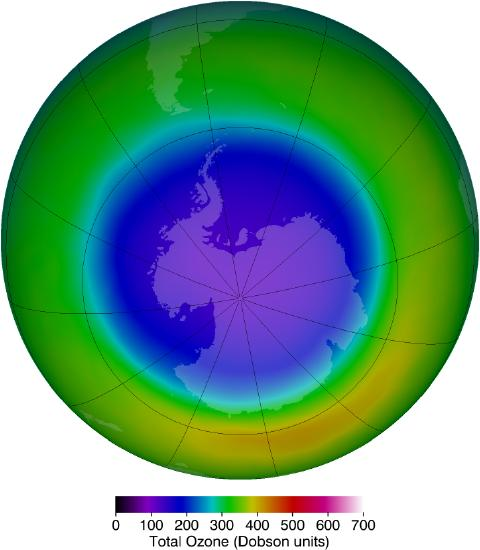
\includegraphics[scale=0.3]{uv}
\end{center}
Ultraviolet means “above violet.” The electromagnetic frequencies of ultraviolet radiation (UV) extend upward from violet, the highest-frequency visible light. Ultraviolet is also produced by atomic and molecular motions and electronic transitions. The wavelengths of ultraviolet extend from 400 nm down to about 10 nm at its highest frequencies, which overlap with the lowest X-ray frequencies. It was recognized as early as 1801 by Johann Ritter that the solar spectrum had an invisible component beyond the violet range. UV rays are important to humans because they help us secrete vitamin D. At the same time they could be carcinogenic if exposed for a long time. UV rays also facilitate the breakdown CFCs(Chloro Flouro Carbons) which directly play a part in the depletion of the ozone layer.
\subsubsection*{X Rays}
\begin{center}
	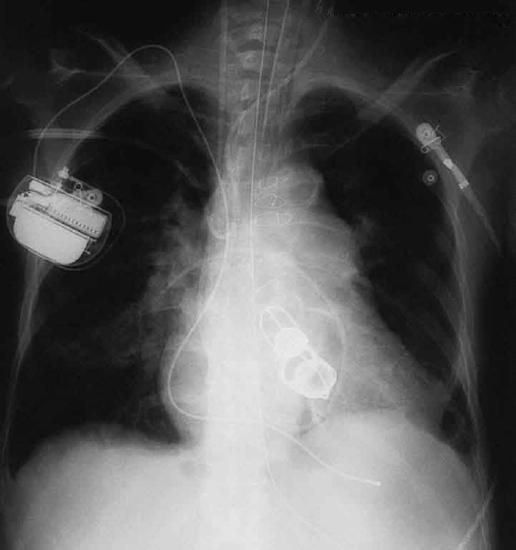
\includegraphics[scale=0.2]{x}
\end{center}
In the mid 19th Century, scientists (such as Faraday) began experimenting with high-voltage electrical discharges in tubes filled with rarefied gases. It was later found that these discharges created an invisible, penetrating form of very high frequency electromagnetic radiation. This radiation was called an X-ray, because its identity and nature were unknown. X-rays have adverse effects on living cells similar to those of ultraviolet radiation, and they have the additional liability of being more penetrating, affecting more than the surface layers of cells. Cancer and genetic defects can be induced by exposure to X-rays. Because of their effect on rapidly dividing cells, X-rays can also be used to treat and even cure cancer. \\ \\
An electron is accelerated in an evacuated tube by a high positive voltage. The electron strikes a metal plate and produces X-rays. Since this is a high-voltage discharge, the electron gains sufficient energy to ionize the atom. After the atom is ionized, it gains an electron and emits energy in form of X rays. Another way X rays could be created is by an electron being slowed by collisions in a material and emitting X-ray radiation. This energetic electron makes numerous collisions with electrons and atoms in a material it penetrates. An accelerated charge radiates EM waves, a second method by which X-rays are created.
\subsubsection*{$\gamma$ Rays}
\begin{center}
	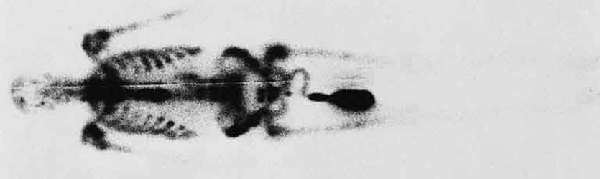
\includegraphics[scale=1.2]{gamma}
\end{center}
Soon after nuclear radioactivity was first detected in 1896, it was found that at least three distinct types of radiation were being emitted. The most penetrating nuclear radiation was called a gamma ray ($\gamma$ ray) (again a name given because its identity and character were unknown), and it was later found to be an extremely high frequency electromagnetic wave. \\ \\
In fact,  Gamma rays are any electromagnetic radiation emitted by a nucleus. This can be from natural nuclear decay or induced nuclear processes in nuclear reactors and weapons. The lower end of the  $\gamma$-ray frequency range overlaps the upper end of the X-ray range, but  $\gamma$ rays can have the highest frequency of any electromagnetic radiation. \\ \\
Gamma rays have characteristics identical to X-rays of the same frequency -- they differ only in source. At higher frequencies,  $\gamma$ rays are more penetrating and more damaging to living tissue. They have many of the same uses as X-rays, including cancer therapy. Gamma radiation from radioactive materials is used in nuclear medicine.












 
\end{document}	